\chapter{Description des monstres}
\section{Niveau 1}
\subsection{Squelette}\label{monster:s6}
\begin{itemize}
  \item \textbf{Apparence :}
  \begin{itemize}
    \item Squelette humain muni de crocs et d'une arme rouillée.
    \item Couvert de bracelets.
  \end{itemize}
  \item \textbf{ Désirs :} protéger le reste de la Tombe des Rois Serpents et tuer tout intrus.
  \item Ne subissent que la moitié des dégâts infligés par les armes perçantes ou tranchantes.
  \item Ils craquent et cliquettent, meurtriers et implacables
\end{itemize}

\SetTblrInner{hspan=minimal, vspan=even}
\begin{osrtable}{X[2]X[1]X[1]X[2]}{0}
  \SetCell[c=4]{bg=black,fg=white} {\bfseries\large\sectionfont Statistiques} & & &\\
  \textbf{CA}          & 7 [12] & \textbf{TACO}        & 19 [0] \\
  \textbf{Attaque}     & \SetCell[c=3]{l} 1D6 (griffes) & &\\
  \textbf{Sauvegardes} & \SetCell[c=3]{l} {\small \textbf{MP}~12 \textbf{B}~13 \textbf{PP}~14 \textbf{S}~15 \textbf{SSB}~16}& &\\
  \textbf{Mouvement} & 18m    & \textbf{Moral} & 12 \\
  \textbf{DV} & 1   & \textbf{XP} & 10 \\
  \textbf{PV} (\hspace*{20pt}) & \SetCell[c=3]{l}\noindent\hdsquares{1} & &\\
  \textbf{PV} (\hspace*{20pt}) & \SetCell[c=3]{l}\noindent\hdsquares{1} & &\\
  \textbf{PV} (\hspace*{20pt}) & \SetCell[c=3]{l}\noindent\hdsquares{1} & &\\
\end{osrtable}

\vfill\
\begin{center}
  \vspace*{0.2\textheight}
  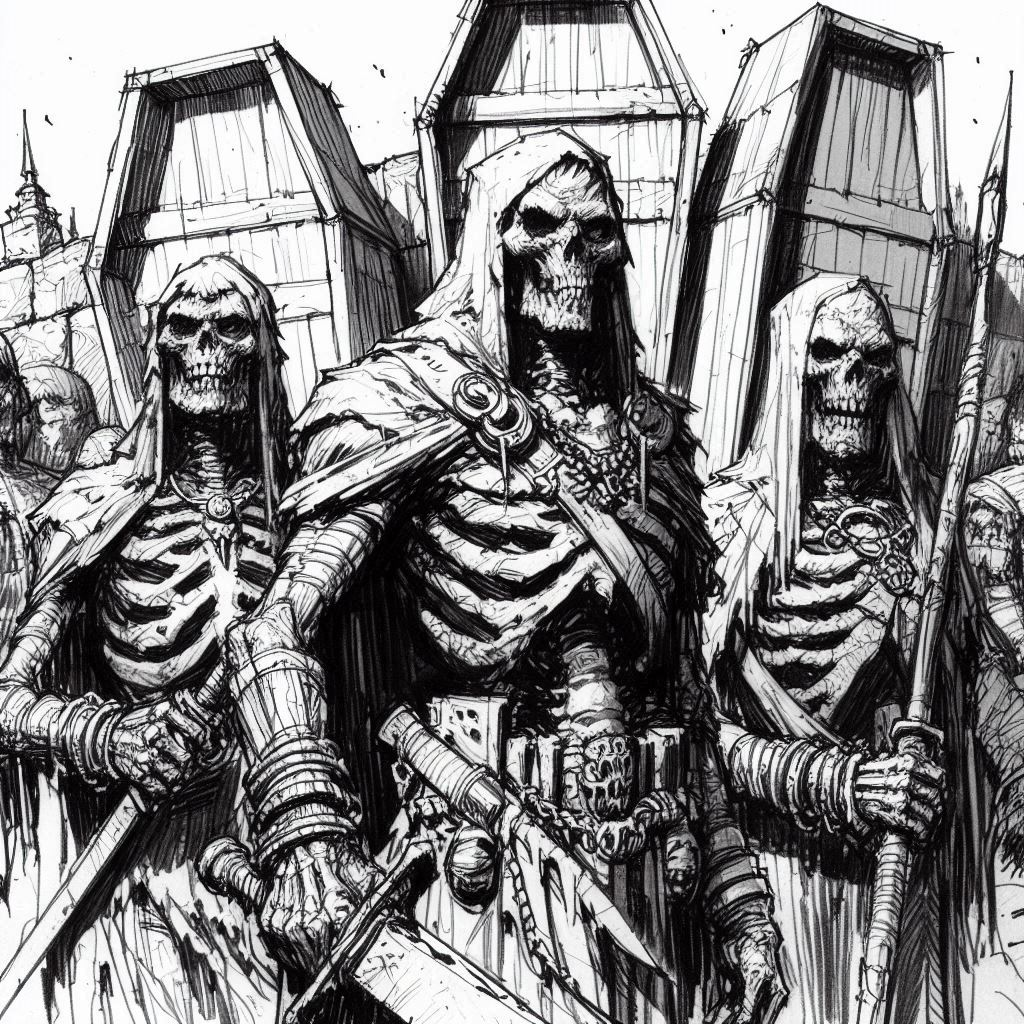
\includegraphics[width=\linewidth]{pics/squelette.jpg}
\end{center}
\vfill

\pagebreak
\section{Niveau 2}
\subsection{Fragments de Momie}\label{monster:s11}
\begin{itemize}
  \item \textbf{Apparence :}
  \begin{itemize}
    \item Bras noircis et décomposés
    \item Doigts acérés
  \end{itemize}
  \item \textbf{ Désirs :}  étrangler des choses, occire les vivants.
\end{itemize}

\SetTblrInner{hspan=minimal, vspan=even}
\begin{osrtable}{X[2]X[1]X[1]X[2]}{0}
  \SetCell[c=4]{bg=black,fg=white} {\bfseries\large\sectionfont Statistiques} & & &\\
  \textbf{CA}          & 7 [12] & \textbf{TACO}        & 19 [0] \\
  \textbf{Attaque}     & \SetCell[c=3]{l} 1D6 (griffes) & &\\
  \textbf{Sauvegardes} & \SetCell[c=3]{l} {\small \textbf{MP}~12 \textbf{B}~13 \textbf{PP}~14 \textbf{S}~15 \textbf{SSB}~16}& &\\
  \textbf{Mouvement} & 18m    & \textbf{Moral} & 12 \\
  \textbf{DV} & 1*   & \textbf{XP} & 13 \\
  \textbf{PV} (\hspace*{20pt}) & \SetCell[c=3]{l}\noindent\hdsquares{1} & &\\
  \textbf{PV} (\hspace*{20pt}) & \SetCell[c=3]{l}\noindent\hdsquares{1} & &\\
\end{osrtable}

\begin{itemize}
\item \textbf{Maladie :}
\begin{itemize}
  \item Maladie putrescente au toucher
  \item Guérison magique inefficace
  \item Guérison naturelle 10x plus longue
  \item Ne peut être éliminée que par magie
\end{itemize}
\item \textbf{Mort-vivant}
\begin{itemize}
  \item Silencieux.
  \item Insensible aux effets affectant les créatures vivantes.
  \item Immunisée contre les sorts affectant ou lisant l'esprit.
\end{itemize}
\end{itemize}

Ils se tortillent, grimpent votre corps et tentent de vous étrangler.

\vfill
%\pagebreak

\subsection{Sparamantur}\label{monster:s13}
\begin{itemize}
  \item \textbf{Apparence :}
  \begin{itemize}
    \item Squelette humain muni de crocs et d'une arme rouillée.
    \item Couvert de bracelets.
  \end{itemize}
  \item \textbf{ Désirs :} protéger le reste de la Tombe des Rois Serpents et tuer tout intrus.
\end{itemize}

\SetTblrInner{hspan=minimal, vspan=even}
\begin{osrtable}{X[2]X[1]X[1]X[2]}{0}
  \SetCell[c=4]{bg=black,fg=white} {\bfseries\large\sectionfont Statistiques} & & &\\
  \textbf{CA}          & 7 [12] & \textbf{TACO}        & 17 [2] \\
  \textbf{Attaque}     & \SetCell[c=3]{l} 1D8 (Hache de bataille) & &\\
  \textbf{Déplacement} & 18m    & \textbf{Moral} & 12 \\
  \textbf{Sauvegardes} & \SetCell[c=3]{l} {\small \textbf{MP}~12 \textbf{B}~13 \textbf{PP}~14 \textbf{S}~15 \textbf{SSB}~16}& &\\
  \textbf{Mouvement} & 18m    & \textbf{Moral} & 12 \\
  \textbf{DV} & 3   & \textbf{XP} & 35 \\
  \textbf{PV} (\hspace*{20pt}) & \SetCell[c=3]{l}\noindent\hdsquares{3} & &\\
\end{osrtable}

\begin{itemize}
  \item Ne subit que la moitié des dégâts infligés par les armes perçantes ou tranchantes.
  \item Il craque et cliquette, meurtrier et implacable
\end{itemize}

\vfill
%\pagebreak

\subsection{Pudding Noir (Franbinzar)}\label{monster:s14}
\begin{itemize}
  \item \textbf{Apparence :}  100 kg de mélasse noire
  \item \textbf{ Désirs :} Se nourrir.
\end{itemize}

\begin{osrtable}{X[2]X[1]X[1]X[2]}{0}
 \SetCell[c=4]{bg=black,fg=white} {\bfseries\large\sectionfont Statistiques} & & &\\
 \textbf{CA}          & 6 [13] & \textbf{TACO}        & 15 [4] \\
 \textbf{Attaque}     & \SetCell[c=3]{l} 2D8 (toucher) & &\\
 \textbf{Sauvegardes} & \SetCell[c=3]{l} {\small \textbf{MP}~10 \textbf{B}~11 \textbf{PP}~12 \textbf{S}~13 \textbf{SSB}~14}& &\\
 \textbf{Mouvement} & 18m    & \textbf{Moral} & 12 \\
 \textbf{DV} &  5   & \textbf{XP} & 300 \\
 \textbf{PV} (\hspace*{20pt}) & \SetCell[c=3]{l}\noindent\hdsquares{5} & &\\
\end{osrtable}

\begin{itemize}
  \item \textbf{Immunité :} Blessé uniquement par le feu, autres: dégâts temporaires
  \item \textbf{Division :} Les attaques qui ne sont pas liées au feu (y compris les sorts) provoquent la division du pudding. Chaque coup crée un nouveau pudding de 1 DV qui inflige 1d6 points de dégâts.
  \item \textbf{Corrosion :} Peut dissoudre le bois ou le métal en un tour (10\% de chances).
  \item \textbf{Collant :} Peut se déplacer sur les murs et les plafonds.
  \item \textbf{Suintement :} Peut s'infiltrer à travers les petits trous et fissures.
  \item \textbf{Régénération :} Si tué, se régénère en 1d20 heures, à moins d'être incinéré.
  \item \textbf{Attaques multiples :} Peut cibler tous les PJ adjacents à chaque round, effectuant un jet d'attaque classique pour chacun.
\end{itemize}

Franbinzar était le dernier roi de la forteresse.

Sa momification ne s'est pas déroulée correctement.
Il s'est transformé en Pudding Noir.

On peut apercevoir 200PO d'anneaux noyés dans sa masse.

\vfill

%\columnbreak

\subsection{Gardien Cobra de Pierre}\label{monster:s19}
\begin{itemize}
  \item \textbf{Apparence :}
  \begin{itemize}
    \item  Chevalier de pierre vêtu d'une armure sculptée.
    \item Une de ses mains manie une imposante épée dentelée.
    \item L'autre est libre au début du combat.
  \end{itemize}
  \item \textbf{ Désirs :}  protéger le reste de la Tombe des Rois Serpents et  tuer les intrus.
\end{itemize}

\begin{osrtable}{X[2]X[1]X[1]X[2]}{0}
  \SetCell[c=4]{bg=black,fg=white} {\bfseries\large\sectionfont Statistiques} & & &\\
  \textbf{CA}          & 3 [16] & \textbf{TACO}        & 15 [4] \\
  \textbf{Attaque}     & \SetCell[c=3]{l} 2D6 (épée dentelée) & &\\
  \textbf{Sauvegardes} & \SetCell[c=3]{l} {\small \textbf{MP}~10 \textbf{B}~11 \textbf{PP}~12 \textbf{S}~13 \textbf{SSB}~14}& &\\
  \textbf{Mouvement} & 18m    & \textbf{Moral} & 12 \\
  \textbf{DV} &  4+1   & \textbf{XP} & 125 \\
  \textbf{PV} (\hspace*{20pt}) & \SetCell[c=3]{l}\noindent\hdsquares{4}~$\square$ & &\\
\end{osrtable}

\textbf{Attaques :} Chaque round, le Gardien Cobra de Pierre peut
appliquer une de ces stratégies :
\begin{enumerate}
  \item \textbf{Appel du Bouclier :}
  Le Gardien appelle à lui un des boucliers couvrant les murs de l'arène.
  \begin{itemize}
    \item 1d6 dégâts (jet de sauvegarde contre la mort pour esquiver) si sur trajectoire
    \item Garde le bouclier (+1 CA)
  \end{itemize}
  \item \textbf{Bond et Impact :}
  Le Gardien bondit à travers les airs puis plonge jusqu'à 6 m de sa position initiale.
  \begin{itemize}
    \item toute créature adjacente : 1d4 dégâts (sauvegarde contre la mort annule).
    \item si dégât : projeté au sol
  \end{itemize}
  \item \textbf{Attaque normale}
\end{enumerate}

\textbf{Stratégies possibles :}
\begin{itemize}
  \item Prendre le Gardien en \textbf{tenaille}
  \item \textbf{Fuir :} Trop imposant pour l'escalier
  \item \textbf{Courir :} suit le PJ tant que détectables
\end{itemize}

\vfill
\pagebreak

\section{Niveau 3}
\subsection{Monstres Errants}\label{monster:n3:errants}
\begin{enumerate}
  \item \textbf{Présage du Basilic.}
  Des cliquetis et grincements d'une chaîne distante traînée sur de la roche et dans la poussière.
  \item \textbf{Présage de Gelées Squelettes.}
  Des bruits de succion résonnant dans le lointain.
  \item \textbf{Présage de Gobelins.}
  \begin{itemize}
    \item Chuchotis, gloussements, grincements de dents et pourléchage de babines.
    \item Le reflet d'yeux rouges dans l'obscurité.
    \item Un fumet de pourriture fongique.
  \end{itemize}
  \item \textbf{Chauve-souris.}
  Nullement hostile, mais effrayante sur le moment.
  Volette de-ci de-là, plane en direction du gouffre.
  \item \textbf{\nameref{monster:n3:araignee}}
  \item \textbf{1d6 \nameref{monster:n3:gob}} en reconnaissance.
  \begin{itemize}
    \item 1d6 autres gobelins fongiques postés au détour du prochain couloir.
  \end{itemize}
  \item  \textbf{1 \nameref{monster:n3:squelgel}.}
  \item  \textbf{1d10+5 \nameref{monster:n3:gob}} parés au combat.\\
  L'un d'eux est muni d'une lance faite de couverts, absurdement peu pratique à manier (1d6 dégâts, allonge)
\end{enumerate}


%\pagebreak
\subsection{Grosse Araignée}\label{monster:n3:araignee}
  \begin{itemize}
  \item De la taille d'un poing.
  \item Cherche à manger des chauves-souris, pas les PJ.
  \item \textbf{Venimeuse : } 1d4 dégâts
  \begin{itemize}
    \item sauvegarde poison annule
  \end{itemize}
  \item \textbf{lâche}
  \item Mets de choix pour les gobelins fongiques.
\end{itemize}

\SetTblrInner{hspan=minimal, vspan=even}
\begin{osrtable}{X[2]X[1]X[1]X[2]}{0}
  \SetCell[c=4]{bg=black,fg=white} {\bfseries\large\sectionfont Statistiques} & & &\\
  \textbf{CA}          & 7 [12] & \textbf{TACO}        & 19 [0] \\
  \textbf{Attaque}     & \SetCell[c=3]{l} 1D3 (morsure) + poison & &\\
  \textbf{Sauvegardes} & \SetCell[c=3]{l} {\small \textbf{MP}~12 \textbf{B}~13 \textbf{PP}~14 \textbf{S}~15 \textbf{SSB}~16}& &\\
  \textbf{Mouvement} & 9m    & \textbf{Moral} & 8 \\
  \textbf{DV} & 1/2   & \textbf{XP} & 5 \\
  \textbf{PV} (\hspace*{20pt}) & \SetCell[c=3]{l}\noindent$\square\square\square\square$ & &\\
\end{osrtable}


\vfill
%\columnbreak
\subsection{Gelée Squelette}\label{monster:n3:squelgel}
\begin{itemize}
  \item \textbf{Apparence :} Un squelette couvert de mucus orange
  \item \textbf{Désirs :}  écraser des crânes et créer plus de gelées squelettes.
\end{itemize}

\SetTblrInner{hspan=minimal, vspan=even}
\begin{osrtable}{X[2]X[1]X[1]X[2]}{0}
  \SetCell[c=4]{bg=black,fg=white} {\bfseries\large\sectionfont Statistiques} & & &\\
  \textbf{CA}          & 7 [12] & \textbf{TACO}        & 19 [0] \\
  \textbf{Attaque}     & \SetCell[c=3]{l} 1D4 (griffes) & &\\
  \textbf{Sauvegardes} & \SetCell[c=3]{l} {\small \textbf{MP}~12 \textbf{B}~13 \textbf{PP}~14 \textbf{S}~15 \textbf{SSB}~16}& &\\
  \textbf{Mouvement} & 9m    & \textbf{Moral} & 12 \\
  \textbf{DV} & 2   & \textbf{XP} & 20 \\
  \textbf{PV} (\hspace*{20pt}) & \SetCell[c=3]{l}N.A. & &\\
  \textbf{PV} (\hspace*{20pt}) & \SetCell[c=3]{l}N.A. & &\\
  \textbf{PV} (\hspace*{20pt}) & \SetCell[c=3]{l}N.A. & &\\
  \textbf{PV} (\hspace*{20pt}) & \SetCell[c=3]{l}N.A. & &\\
\end{osrtable}

\begin{itemize}
  \item Immunisés à tous dommages.
  \item \textbf{Solutions possibles:}
  \begin{itemize}
    \item Fuir,
    \item les faire pétrifier par le \textbf{\nameref{monster:n3:basilic}},
    \item les précipiter dans le gouffre,
    \item les attacher
    \item les enfermer dans une salle
    \item les précipiter en \textbf{\nameref{n3:s25}} ou \textbf{\nameref{n3:s37}}
  \end{itemize}
  \item Sortent des fosses / se libérent des cordes (temps variable).
  \item \textbf{4} gelées squelettes en tout
  \begin{itemize}
    \item Vaincue : retirer de la \textbf{Table des \nameref{monster:n3:errants}}
  \end{itemize}
  \item \textbf{Contagion:} Toute victime (tuée) devient une gelée squelette en 10 minutes.
  \begin{itemize}
    \item \textbf{\nameref{monster:n3:gob}} immunisés.
  \end{itemize}
\end{itemize}


\vfill

\subsection{Gobelins Fongiques}\label{monster:n3:gob}
\SetTblrInner{hspan=minimal, vspan=even}
\begin{osrtable}{X[2]X[1]X[1]X[2]}{0}
  \SetCell[c=4]{bg=black,fg=white} {\bfseries\large\sectionfont Statistiques} & & &\\
  \textbf{CA}          & 6 [13] & \textbf{TACO}        & 19 [0] \\
  \textbf{Attaque}     & \SetCell[c=3]{l} 1D6 (arme) & &\\
  \textbf{Sauvegardes} & \SetCell[c=3]{l} {\small \textbf{MP}~14 \textbf{B}~15 \textbf{PP}~16 \textbf{S}~17 \textbf{SSB}~18}& &\\
  \textbf{Mouvement} & 18m    & \textbf{Moral} & 7 \\
  \textbf{DV} & 1-1   & \textbf{XP} & 5 \\
  \textbf{PV} (\hspace*{20pt}) & \SetCell[c=3]{l}\noindent\hdsquares{1} & &\\
  \textbf{PV} (\hspace*{20pt}) & \SetCell[c=3]{l}\noindent\hdsquares{1} & &\\
  \textbf{PV} (\hspace*{20pt}) & \SetCell[c=3]{l}\noindent\hdsquares{1} & &\\
  \textbf{PV} (\hspace*{20pt}) & \SetCell[c=3]{l}\noindent\hdsquares{1} & &\\
  \textbf{PV} (\hspace*{20pt}) & \SetCell[c=3]{l}\noindent\hdsquares{1} & &\\
  \textbf{PV} (\hspace*{20pt}) & \SetCell[c=3]{l}\noindent\hdsquares{1} & &\\
  \textbf{PV} (\hspace*{20pt}) & \SetCell[c=3]{l}\noindent\hdsquares{1} & &\\
\end{osrtable}

\begin{itemize}
  \item \textbf{Apparence :}
  \begin{itemize}
    \item pâles et rabougris,
    \item \'Enorme tête ovale
    \item Plein de dents et deux petits yeux rouges beaucoup trop près l'un de l'autre.
    \item Texture évoque une purée de pommes de terre à la colle blanche.
    \item Portent sur eux des couverts de  table.
  \end{itemize}
  \item \textbf{ Désirs :} un roi, à manger, des choses qui brillent, encore à manger
  \item \textbf{Non hostiles :} ils cherchent seulement à couronner quelqu'un Roi des Gobelins (Initialement)
  \item \textbf{Dialecte :} gobelin cliquetant et limité.
  \item Aisément \textbf{corruptibles}
  \item Si PJ hostiles:
  \begin{itemize}
    \item \textbf{Fuite}
    \item \textbf{Embuscades} récurrentes
    \item Sournois et patients
    \item Escaladent (lentement) les murs : surprendre les aventuriers en leur plongeant dessus
    \item Seaux d'eau pour éteindre les torches
    \item Cordes pour emmêler les combattants
    \item Tirent profit des pièges du donjon
    \item De nuit, harcèlent le campement
  \end{itemize}
  \item \textbf{Roi des gobelins :} destin
  \begin{itemize}
    \item suivi jusqu'à la pleine lune
    \item puis assailli, traîné jusqu'à un autel au sommet d'une colline et éventré
  \end{itemize}
  \item \textbf{Connaissances :}
  \begin{itemize}
    \item Peuvent avertir au sujet du \textbf{\nameref{monster:n3:basilic}}
    \item Ignorent l'existence du \textbf{\nameref{n3:s39}}
    \item Ignorent tout des niveaux supérieurs : bloqués par le \textbf{\nameref{monster:s19}}
  \end{itemize}
\end{itemize}

La nuit venue, ils utilisent \textbf{\nameref{n3:s41}} pour se faufiler jusqu'à l'extérieur.

À moins que \textbf{\nameref{n3:s48}} ne soit incendiée, le nombre de gobelins dans le donjon sera toujours "beaucoup trop de gobelins".

Les gobelins fongiques sont des rats de laboratoire parvenus à s'échapper.
Bien que \textbf{\nameref{monster:n3:xiximanter}} ne s'oppose pas à ce qu'on les lui rende, ils ne lui sont pas d'une grande utilité.

\vfill
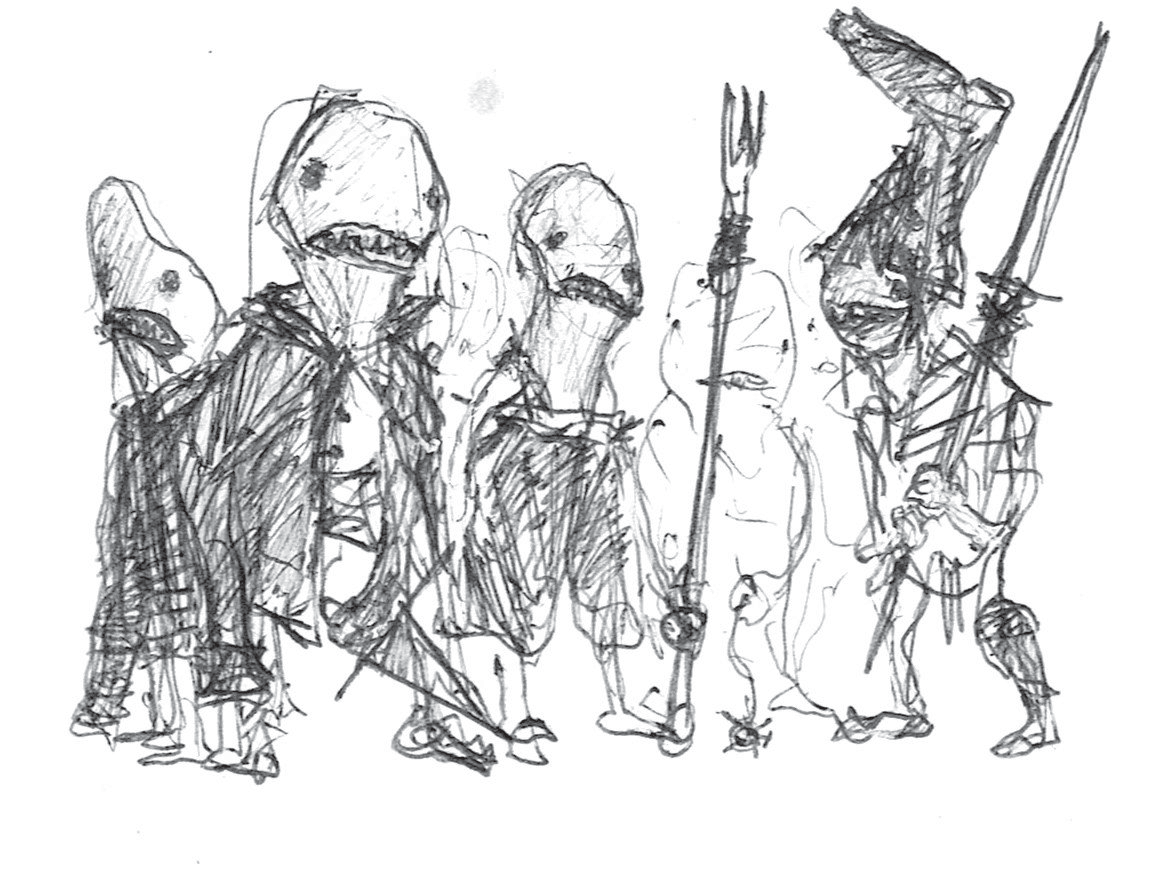
\includegraphics[width=\columnwidth]{pics/gob.png}

\pagebreak
\subsection{Succube}\label{monster:n3:succube}
\begin{itemize}
  \item \textbf{Apparence :}  Jeune botaniste de la race du premier PJ qu'il aperçoit, et de sexe approprié
  \item \textbf{ Désirs :}
  \begin{itemize}
    \item \textbf{Recharger ses réserves :} embrasser un PJ (drain)
    \item \textbf{S'échapper :} pousser quelqu'un à s'approcher et franchir le cercle de confinement.
  \end{itemize}
\end{itemize}

\SetTblrInner{hspan=minimal, vspan=even}
\begin{osrtable}{X[2]X[1]X[1]X[2]}{0}
  \SetCell[c=4]{bg=black,fg=white} {\bfseries\large\sectionfont Statistiques} & & &\\
  \textbf{CA}          & 2 [17] & \textbf{TACO}        & 14 [+5] \\
  \textbf{Attaque}     & \SetCell[c=3]{l} 1D3 (2 $\times$ griffes) & &\\
  \textbf{Sauvegardes} & \SetCell[c=3]{l} {\small \textbf{MP}~10 \textbf{B}~11 \textbf{PP}~12 \textbf{S}~13 \textbf{SSB}~14}& &\\
  \textbf{Mouvement} & 18m    & \textbf{Moral} & 10 \\
  \textbf{DV} & 6*  & \textbf{XP} & 500 \\
  \textbf{PV} (\hspace*{20pt}) & \SetCell[c=3]{l}\noindent\hdsquares{6} & &\\
\end{osrtable}

\begin{itemize}
  \item \textbf{Immunité :} Pétrification, Feu et armes non magiques
  \item \textbf{Drain d'énergie :} Un baiser draine d'un niveau. Sauvegarde contre la mort annule
  \item \textbf{Sorts :} Charme-personne, Image miroir
  \item Son nom véritable (\textbf{Baltoplate}) figure  sur un parchemin en salle \textbf{\nameref{n2:s15}}
  \item Fuit tout combat, refuse de s'y risquer.
  \item Ne revient pas ensuite.
  \item Si doit marchander pour sa vie / liberté, , il peut proposer de :
  \begin{itemize}
    \item Détecter les poisons,
    \item Révéler d'anciens secrets
    \item Tuer n'importe quelle personne mortelle que les PJ peuvent nommer
  \end{itemize}
  \item Patient et fourbe, mais tient toujours parole
\end{itemize}

\vfill\
\begin{center}
  \vspace*{0.2\textheight}
  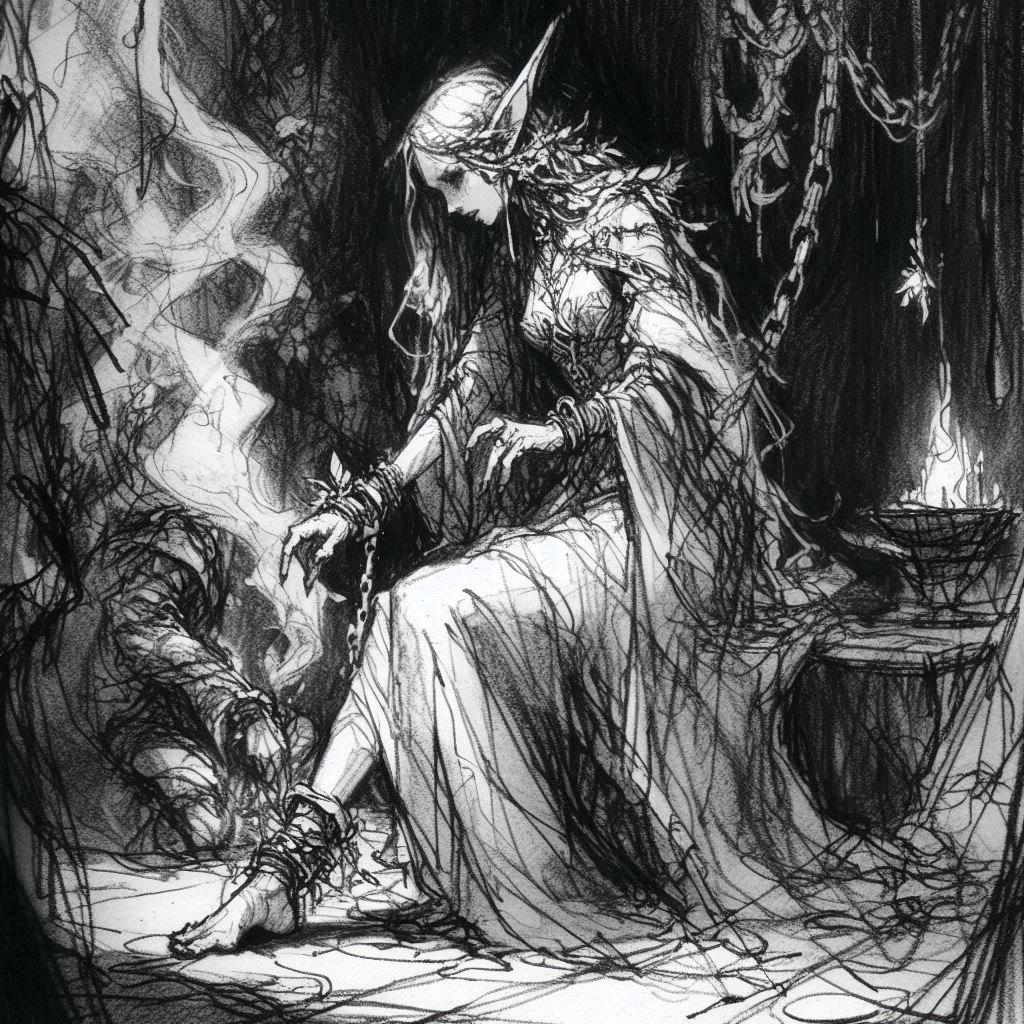
\includegraphics[width=\linewidth]{pics/succube.jpg}
\end{center}
\vfill

\pagebreak
\subsection{Basilic}\label{monster:n3:basilic}
\begin{itemize}
  \item \textbf{Apparence :}
  \begin{itemize}
    \item titanesque lézard octopède à tête crocodilienne aplatie et pleine de dents.
    \item \OE illères de bronze vissées dans le crâne
    \item Collier autour du cou, juste devant sa première paire de pattes.
  \end{itemize}
  \item \textbf{ Désirs :} nourriture, chaleur et liberté.
\end{itemize}

\SetTblrInner{hspan=minimal, vspan=even}
\begin{osrtable}{X[2]X[1]X[1]X[2]}{0}
  \SetCell[c=4]{bg=black,fg=white} {\bfseries\large\sectionfont Statistiques} & & &\\
  \textbf{CA}          & 4 [15] & \textbf{TACO}        & 13 [+6]  \\
  \textbf{Attaque}     & \SetCell[c=3]{l} 1 morsure (1d10 + pétrification) & &\\
  \textbf{Attaque}     & \SetCell[c=3]{l} 1 regard (pétrification)  & &\\
  \textbf{Attaque}     & \SetCell[c=3]{l} 1 coup de queue (1D8 + projection)  & &\\
  \textbf{Sauvegardes} & \SetCell[c=3]{l} {\small \textbf{MP}~10 \textbf{B}~11 \textbf{PP}~12 \textbf{S}~13 \textbf{SSB}~14}& &\\
  \textbf{Mouvement} & 18m    & \textbf{Moral} & 10 \\
  \textbf{DV} & 6+1*  & \textbf{XP} & 950 \\
  \textbf{PV} (\hspace*{20pt}) & \SetCell[c=3]{l}\noindent\hdsquares{6}~$\square$ & &\\
\end{osrtable}

\begin{itemize}
  \item \textbf{Surprise :} Les personnages surpris par le basilic subissent une attaque de son regard pétrifiant.
  \item \textbf{Éviter son regard :} Une personne qui cherche à combattre le basilic en évitant son regard subit un malus de –4 pour toucher, tandis que le basilic bénéficie d'un bonus de +2.
  \item \textbf{Utiliser un miroir :} Le reflet du basilic est inoffensif. Se battre en regardant dans un miroir inflige un malus de –1 à l'attaque. Si le basilic voit son propre reflet (2 chances sur 6), il doit effectuer un jet de sauvegarde ou être pétrifié.
  \item \textbf{Pétrification :}
  \begin{itemize}
    \item \textbf{Simple coup d'\oe il:} légère sensation de pression
    \item \textbf{Fixe 1 round :} les membres sont lents, pesants, les pensées ralentissent.
    Immobile et -4 à la défense (sauvegarde contre la Pétrification annule).
    L'effet prend fin dès que le basilic détourne le regard.
    \item \textbf{Fixe 2 rounds :} Transformé en pierre (sauvegarde contre la Pétrification annule).
    Si réussite, reste cependant fixée sur place.
  \end{itemize}
  \item \OE illères peuvent être fermées
  \item \textbf{Comportement :}
  \begin{itemize}
    \item \textbf{Affamé (par défaut) :} se mouvant lentement dans l'obscurité, humant l'air, cherchant à identifier une proie isolée.
    Il se tient sur ses gardes si le groupe déclenche le piège du \textbf{\nameref{n3:s35}} ou ouvre la porte du \textbf{\nameref{n3:s39}}.
    \item \textbf{En digestion (si repus) :} lové dans un coin, dos au  mur, la tête relevée et paré à réagir.
    3 chances sur 6 d'être endormi.
    \item \textbf{Curieux (si repus) :} humant l'air, dodelinant de la tête pour éviter de pétrifier quelque chose par accident.
    Il peut reconnaître ceux qui l'ont nourri à l'odeur (lézard apprivoisé, il a appris  à ne pas mordre la main qui le nourrit).
    \item \textbf{Rage (si effrayé ou blessé) :} bondit en arrière de 3 m, dresse la queue et charge une cible dans le même tour.
    Celle-ci doit effectuer un jet de sauvegarde contre la paralysie .
  \end{itemize}
  \item Repus avec :
  \begin{itemize}
    \item 30 rations de voyage
    \item 2 humains normaux
    \item 1 cheval
    \item 6 gobelins fongiques
  \end{itemize}
\end{itemize}

Les mages et alchimistes accordent une grande valeur aux yeux du basilic (300 PO chaque).

Ses glandes salivaires contiennent l'équivalent de 2 potions de "Transmutation de la Pierre en Chair".

Son squelette pierreux peut se revendre 1000 PO, ou 300 PO pour la tête seule.

Vivante, la bête peut s'échanger contre 10.000 PO dans une ménagerie, le double si elle est domestiquée.

\vfill
\pagebreak
\subsection{Xiximanter}\label{monster:n3:xiximanter}
\begin{itemize}
  \item \textbf{Apparence :}
  \begin{itemize}
    \item Buste humain desséché
    \item Queue de serpent squelettique.
    \item Haillons d'une robe de mage
    \item Charmes et amulettes pendent à son cou.
    \item Deux yeux rouges, brûlant telles des aiguilles de feu.
    \item Deux crocs acérés.
    \item Toujours poli.
  \end{itemize}
  \item \textbf{ Désirs :}  êtres vivants, sorts, ingrédients rares pour potions
\end{itemize}

\SetTblrInner{hspan=minimal, vspan=even}
\begin{osrtable}{X[2]X[1]X[1]X[2]}{0}
  \SetCell[c=4]{bg=black,fg=white} {\bfseries\large\sectionfont Statistiques} & & &\\
  \textbf{CA}          & 1 [18] & \textbf{TACO}        & 11 [+8]  \\
  \textbf{Attaque}     & \SetCell[c=3]{l} 1 griffes (1d8 + paralysie) & &\\
  \textbf{Sauvegardes} & \SetCell[c=3]{l} {\small \textbf{MP}~6 \textbf{B}~7 \textbf{PP}~8 \textbf{S}~9 \textbf{SSB}~10}& &\\
  \textbf{Mouvement} & 18m    & \textbf{Moral} & 10 \\
  \textbf{DV} & 10***  & \textbf{XP} & 3700 \\
  \textbf{PV} (\hspace*{20pt}) & \SetCell[c=3]{l}\noindent\hdsquares{10} & &\\
\end{osrtable}

\begin{itemize}
  \item \textbf{Mort-vivant :} Silencieux jusqu'à l'attaque.
  Immunisé contre les effets qui affectent les créatures vivantes (par exemple le poison).
  Immunisé contre les sorts affectant l'esprit (par exemple, charme, immobilisation, sommeil).
  \item \textbf{Immunité :} Armes non magiques, électricité, froid, tous les sorts qui provoquent la métamorphose, la folie, la mort.
  \item \textbf{Aura de peur :} Xiximanter peut décider d'activer/désactiver son aura de peur.
  Ceux qui le voient doivent effectuer un jet de sauvegarde contre les sorts ou fuir pendant 2d6 tours.
  Les personnages de niveau 4 ou plus sont immunisés.
  \item \textbf{Griffe paralysante :} sauvegarde contre la paralysie ou paralysé pendant 6 tours.
  \item \textbf{Sorts mémorisés:} Comme un mage de niveau 10.
  \begin{itemize}
    \item \textbf{Niveau 1 :} Projectile magique, Sommeil, Charme-personne
    \item \textbf{Niveau 2 :} Invisibilité, ESP, Détection de l'invisible
    \item \textbf{Niveau 3 :} Boule de feu, Foudre, Paralysie
    \item \textbf{Niveau 4 :} Mur de feu, Confusion, Allométamorphose
    \item \textbf{Niveau 5 :} Débilité mentale, Téléportation
  \end{itemize}
  \item \textbf{Attitude :}
  \begin{itemize}
    \item Raisonnable, avenant (\emph{"Bonjour, bipèdes"})
    \item Besoin de créatures vivantes, de préférence intelligentes, des sorciers dans l'idéal.
    \item Les distille pour élaborer ses potions
    \item Croit fermement être sur le point de faire une découverte révolutionnaire
    \item Croit que la ville des hommes-serpents s'étend toujours à la surface, que la tombe est pleine de prêtres
    \item Entre dans une rage folle si confronté à la réalité
  \end{itemize}
\end{itemize}